\documentclass{article}

\usepackage[utf8]{inputenc}
\usepackage{fancyhdr}
\usepackage{geometry}
\usepackage[frenchb]{babel}
\usepackage{libertine}
\usepackage[pdftex]{graphicx}
\usepackage{hyperref}
\usepackage{slashbox}
\usepackage[T1]{fontenc}
\usepackage{multirow}
\usepackage{graphicx}
\usepackage{array,multirow,makecell}
\setcellgapes{1pt}
\makegapedcells
\newcolumntype{R}[1]{>{\raggedleft\arraybackslash }b{#1}}
\newcolumntype{L}[1]{>{\raggedright\arraybackslash }b{#1}}
\newcolumntype{C}[1]{>{\centering\arraybackslash }b{#1}}
\geometry{a4paper}
\geometry{top=3cm, bottom=3cm, left=3.5cm, right=3.5cm}



\begin{document}

\large
\begin{titlepage}
		\title{Rapport de la deuxième  soutenance : Lucidity by the Chamallow}
		
		\author{CLAUS Marion -  DELECROIX Thomas - GINANE Charles - MARCHAUD Laurent} 

		
\end{titlepage}
\pagestyle{fancy}
\lhead{The Chamallow}
\rfoot{EPITA infosup}
\renewcommand{\footrulewidth}{0.4pt}
\rhead{Rapport de la première soutenance}

 \begin{titlepage}
\centering
\maketitle
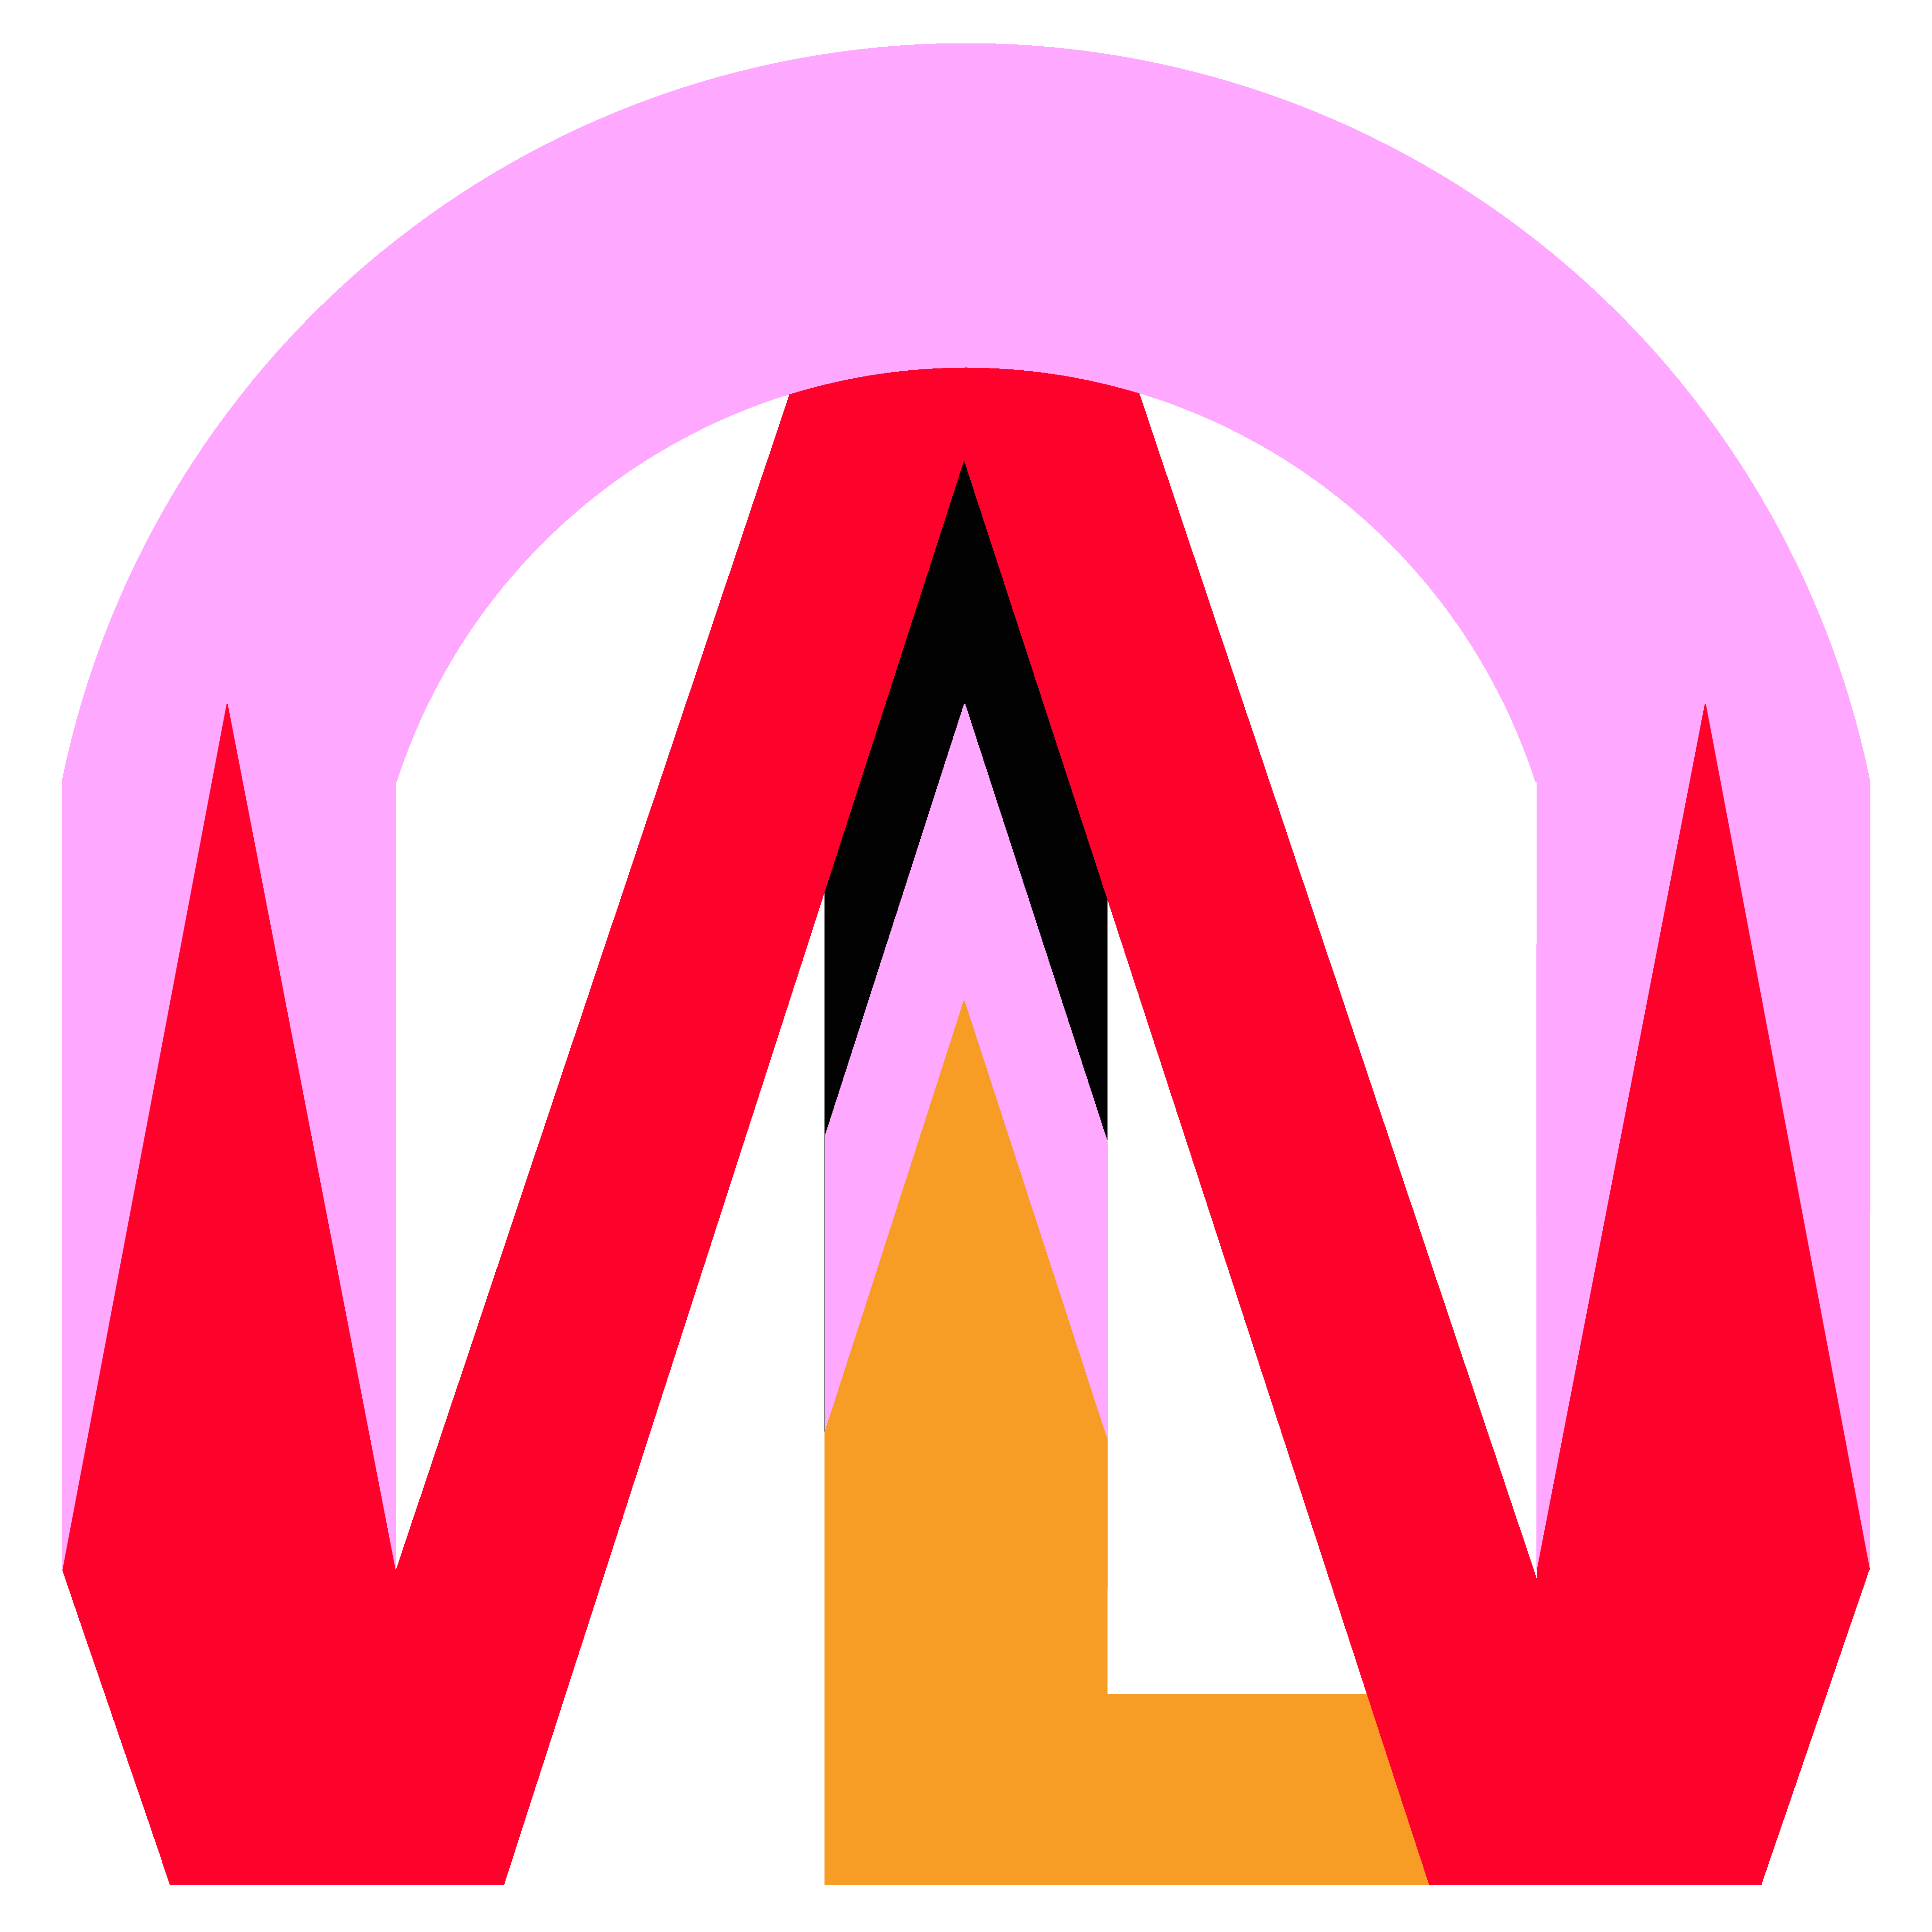
\includegraphics[scale=0.1]{Logo.png}

  \end{titlepage}


\tableofcontents

\newpage

\section{Introduction}

\quad

\quad

    Mercredi 16 mars, 17h00, Epita, Villejuif. Fin de la première soutenance pour The Chamallow. Cela s’est bien passé, mais il ne faut pas s’arrêter en si bon chemin, le jeu n’est pas fini. C’est ainsi que notre groupe a continué ce long et périlleux voyage. Il est maintenant temps de faire notre rapport d’avancement. Dans un premier temps, nous vous rappelerons comment est composé notre groupe et de la mission que nous nous sommes fixée. Puis nous vous présenterons les objectifs que nous devions atteindre pour ce second raid, ce qui a vraiment été réalisé, ainsi que notre réparttion des tâches. Ensuite nous verrons nos objectifs pour notre dernier raid et l’avancement de notre projet, et pour finir notre multijoueur.
Nous vous souhaitons une agréable lecture 


\quad

\quad


\begin{centering}


\textbf {The Chamallow}

\end{centering}

\quad

\quad

\begin{centering}

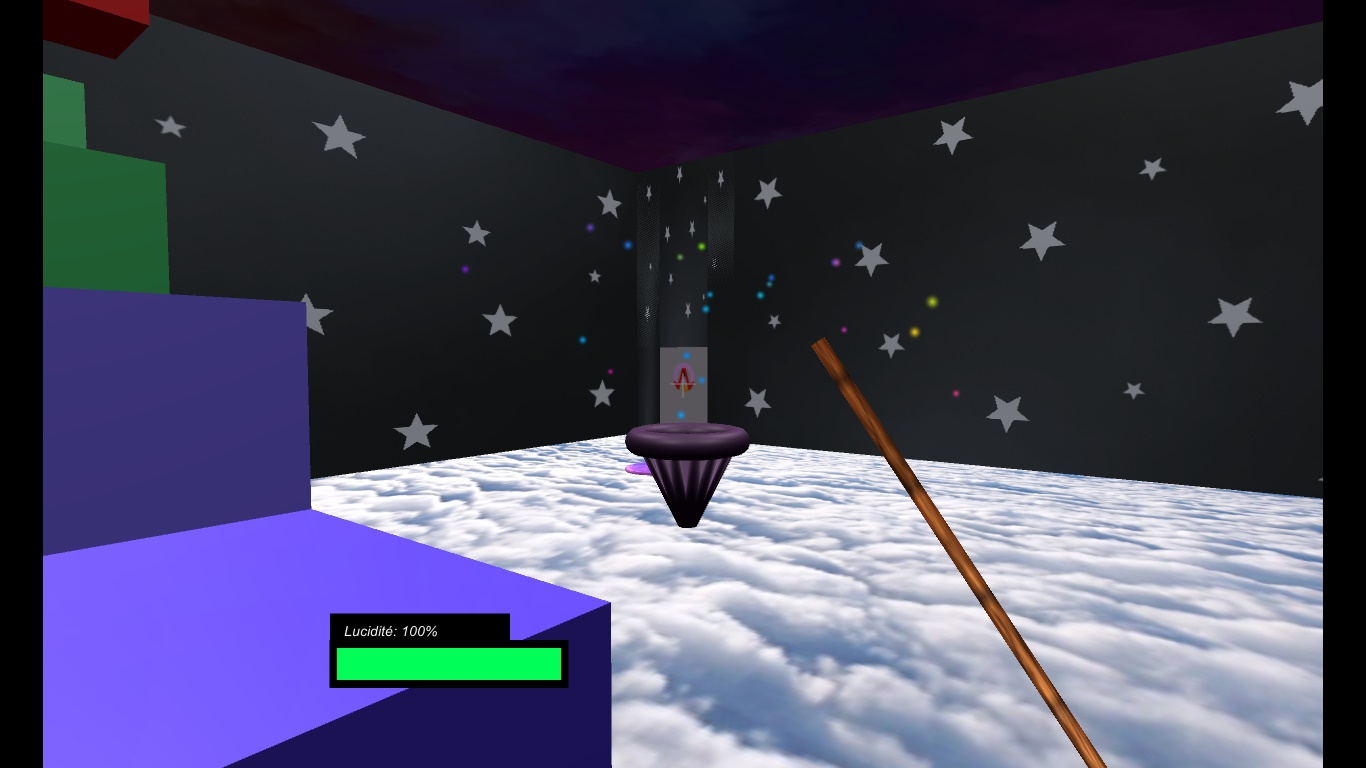
\includegraphics[scale = 0.4]{Portelogo.png}

\quad

\textit{Figure 1 : Pièce du niveau mutli avec une surce de lucidité et une porte}

\end{centering}


\quad


\newpage



\section{Rappel du projet :}

\quad

\quad

Avant de commencer, je juge judicieux de faire un rappel de notre groupe ainsi que de notre projet

	\subsection{Présentation du groupe :}

\quad

\quad

Le groupe “The Chamallow”  est composé de 4 membres. Il est composé de  : 

\quad
- Marion “Santa “ CLAUS  qui s’est occupée de la conception du monde en créant la map du premier niveau et second niveau en solo et le premier en multijoueur et aussi du moteur graphique.

\quad
- Thomas “Tetra” DELECROIX notre chef de projet , qui s’est chargé du moteur physique et la synchronisation du reseau.

\quad
Charles “Gigi” GINANE qui a géré le gameplay tel que l’HUD (ou l’ATH)  et aussi des son du jeu.

\quad
Laurent “Aluxima” MARCHAUD qui s’est occupé des sons et principalement du site du projet ainsi que le reseau.

\quad

\quad


	\subsection{présentation du projet :}

\quad

\quad

Le projet Lucidity est un jeu développé sous Unity, ce jeu à la première personne se base sur la réflexion / puzzle et l’interaction avec le décor afin de trouver la solution et d’arriver au terme du niveau. Il se base sur deux jeux plus ou moins connus, tels que “Portal” et “Qube”.

Notre environnement est constitué de salles closes dans lesquelles le joueur doit effectuer une suite d’actions en interaction avec le décor lui permettant de sortir de la salle et de passer à un niveau supérieur. Pour l'interaction avec le décor, cela se fait grâce à la “Lucidité”, la ressource primaire du jeu. Elle est contenable en quantité limitée dans une bouteille spéciale que le joueur transportera dans son dos. Cette ressource peut être récoltée au niveau des sources, rares, présentes qu’à certains endroits de la carte. Une fois que le personnage n’a plus de Lucidité, il doit recommencer à partir du dernier checkpoint.


\newpage

	\subsection{Nos attentes par rapport au projet :}

\quad

\quad

Nous avons de multiples attentes par rapport à ce projet.

La première est d’avoir une première expérience sur le travail de groupe sur un projet, de savoir ce que c’est .

La deuxième est d’améliorer les connaissances de chacun dans différents domaines tel que le code ou alors l’organisation du projet. De plus, cela nous permet à chacun de partager nos connaissances ce qui encourage la cohésion de groupe 

Enfin, notre dernière attente est de prendre confiance en nous pour le reste de notre cursus et de pouvoir travailler en groupe.

\newpage


\section{Les objectifs pour la deuxième soutenance}

\quad

Nous allons maintenant vous montrer la répartition de nos objectifs par membre du groupe ainsi que  nos objectifs prévus par le cahier des charges pour cette deuxième soutenance.Et ensuite nous ferons le bilan sur ce qui a été fait durant cette période à savoir entre la première soutenance et la deuxième soutenance.

\quad

	\subsection{Rappel des objectifs :}

\quad

\underline{\textbf{Légende de la figure 2:}} : 

\quad
	   -  -     : Pas de participation

 \quad
	- X     : Faible implication

 \quad
	- XX   : Moyenne implication

 \quad
	- XXX : Forte implication 

\quad

\quad 

\begin{tabular}{|c||c|c|c|c|}
\hline Domaine / Nom & Laurent & Charles & Marion & Thomas \\ 
\hline Moteur graphique & - & - & XX & X\\
\hline Moteur physique & - & - & X & XX\\
\hline Site & XXX & X & - & -\\
\hline Réseau & X & - & - & XXX\\
\hline Gameplay & - & XXX & X & -\\
\hline Conception du monde & X & - & XX & -\\
\hline Son & X & XX & - & -\\
\hline
\end {tabular}

\quad

\begin{center}

\textit{Figure 2 : Tableau de répartitions des tâches par membre}

\end{center}

\quad

\underline{\textbf{Légende de la figure 3:}} : 

\quad
	   -  -     : Non commencée

 \quad
	- +     : Objectif peu avancée

 \quad
	- ++   : Objectif moyennement avancée

 \quad
	- +++ : Objectif finie 

\quad

			\begin{tabular}{|c|c|c|c|}
\hline Domaine  & 2ème soutenance \\
\hline Moteur graphique & ++\\
\hline Moteur physique & +++\\
\hline Site & +++ \\
\hline Réseau & ++ \\
\hline Gameplay & ++\\
\hline Conception du monde & ++\\
\hline Son & ++\\
\hline Finalisation &++\\
\hline
			\end {tabular}

\quad

\quad

\begin{centering}

\textit{Figure 3 : Tableau des objectis pour la deuxième soutenance}

\end {centering}


	\subsection{Ce qui a été fait entre la première soutenance et la deuxième soutenance :}


\quad

\quad

Le plus gros travail qui a été réalisé entre les deux soutenances a été le réseau. En effet, Thomas et Laurent ont passé énormément de temps à configurer le réseau pour qu’il fonctionne. Ils se sont occupés de gérer quand les joueurs se connectent et quittent, quand un joueur ouvre une salle, les autres puissent la rejoindre et inversement.

Ils ont aussi adapté les scripts du mode solo pour le multijoueur car le réseau ne prend pas les mêmes scripts étant donné qu’il y a plusieurs joueurs qui se connectent et non que un seul, du coup il y a beaucoup plus de choses à régler. ils ont donc adapté le solo pour le multijoueur.


Laurent a aussi fini le site internet du jeu (Lucidity.fr) où les utilisateurs pourront maintenant mettre des commentaires à propos du jeu.
Marion et Charles ne sont pas restés à les regarder travailler durement. Marion s’est occupée de créer la map multijoueur et la map du niveau 2 tout en appliquant les quelques idées de Charles pour les maps. Marion s’est aussi occupée de créer des textures adaptées à l’environnement du jeu et de les appliquer aux différents niveaux, elle a aussi adapté quelques scripts, notamment celui pour les plateformes, aux autres niveaux afin qu’ils puissent fonctionner sans problème. 
Charles, lui, s’est chargé d’améliorer le gameplay tout ça en améliorant le HUD, il a rajouté plus de textes qui permettent de guider le joueur vers la fin du niveau par le biais de texte qui s’affiche à l’écran du joueur pour lui donner les objectifs à accomplir pour finir le niveau. Charles a aussi géré les sons, pour cela il a ajouté une musique aux différentes actions et aussi au menu principal pour donner une ambiance un peu plus vivante au jeu. Il a aussi implémeté différents sons au sein du jeu pour que ce soit plus interactif et aussi pour aider le joueur (exemple : son dès qu’il a accompli une objectif ou qu’il a rempli sa barre de lucidité).

De ce fait, Charles a débuté le dernier domaine à travailler qui n’est autre que la finalisation du projet en finissant au mieux le premier niveau.

Au terme de cette deuxième soutenance, nous avons atteint l’ensemble de nos objectifs fixés par le cahier des charges. Nous n’avons pas d’avance particulière, nous préferons ne pas nous précipiter et finir à temps nos objectifs.



\newpage

	\subsection{Ce qu'il nous reste à faire}

\quad

\quad


On peut maintenant dire que le plus gros du travail a été fait. En effet, le réseau est maintenant en place grâce à Laurent et Thomas, qui vont l’améliorer au mieux pour que le multijoueur soit de bonne qualité.

Marion va s’occuper de faire de nouvelles maps pour le multijoueur et pour le solo, elle a déjà quelques idées sur le sujet.

Quant à Charle, il va se charger de la finalisation du projet, mais aussi de l’amélioration des sons en ajoutant plus de sons et de musiques relatif au jeu. Il va aussi améliorer au mieux le gameplay. Il aidera aussi Marion à trouver des idées pour les futurs maps du jeu.

\quad

\quad

\newpage


\section{Qui a fait quoi ? :}

\quad

Dans cette troisième partie, chaque membre du groupe va présenter ce qu'il a fait entre les deux soutenances, il va ensuite présenter ce qu'il reste avant de donner son ressenti en conclusion personnelle.


	\subsection{Marion "Santa" CLAUS :}

\quad


		\subsubsection{Ce qui a été fait :}

\quad 

\quad

Lors de la dernière soutenance, j’avais présenté une map pour le mode solo qui était composée de deux parties : un labyrinthe de pièces et une partie avec que des plateformes. Pour cette soutenance, je me suis essentiellement occupée de créer deux nouvelles maps. La première est pour le niveau 2 en mode un joueur. Elle aussi est divisée en deux parties. Il y a d’abord un labyrinthe de plateformes qui apparaissent au fur et à mesure de l’avancée du joueur, dans lequel il faut trouver trois boutons. Ces derniers permettent de révéler les dernières plateformes qui relient le joueur à la deuxième parties de la map. Dans celle-ci, le joueur est sur une plateforme qu’il peut bouger grâce aux clips. Son objectif est alors de se déplacer entre des murs pour atteindre un escalier arc-en-ciel qui amène à la sortie. La seconde est une map créée pour le mode multijoueur, de manière à ce que les deux joueurs dépendent l’un de l’autre doivent s’entraider. Comme les autres maps, elle est organisée en deux fractions. Dans un premier temps, les joueurs ont un parcours de plateformes au bout duquel il y a deux boutons qui affichent les plateformes reliant le joueur à la deuxième partie de la map. Dans celle-ci, les joueurs doivent se séparer et chacun des joueurs doit trouver une bouton qui dévoile deux plateformes qui permettent au coéquipier d’accéder à la porte de sortie. La partie se termine quand les deux joueurs sont au niveau de la sortie. De plus avec Charles, nous avons élaboré les points d’apparition que nous utilisons dans la map du niveau 2 en mode solo pour faire apparaître la map au fur et à mesure que le joueur avance. J’ai aussi revu certaines textures, c’est ainsi que l’on peut voir le logo de notre groupe sur les portes.


\quad

\quad

		\subsubsection{Ce qu'il reste à faire :}

\quad

\quad

Pour la soutenance finale, il me reste encore à faire deux maps : une pour le niveau 3 en mode solo et une pour le niveau 2 en mode multijoueur. De plus, je dois créer un personnage qui pourra remplacer la capsule qui nous sert de joueur.

\quad

\quad

		\subsubsection{Conslusion personnelle :}

\quad

\quad

Pour cette deuxième soutenance, je suis satisfaite de l’avancement de notre jeu. De plus, je pense que le groupe a bien évolué et que nous nous répartissons mieux les tâches.
\quad

\quad


\quad

\begin{centering}

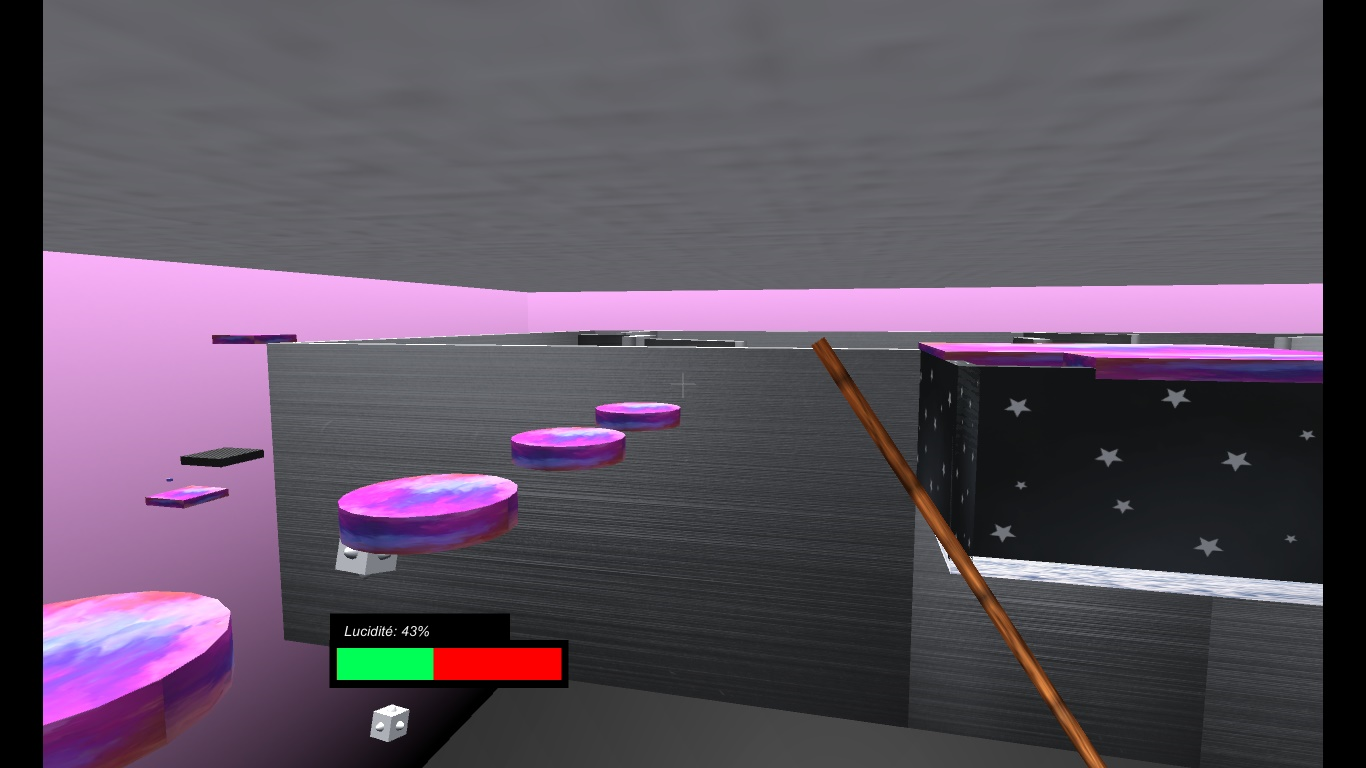
\includegraphics[scale = 0.4]{vuemulti.png}

\quad

\textit{Figure 4 : Vue d'ensemble de la map multijoueur }

\end{centering}


\quad

\begin{centering}

\includegraphics[scale = 0.4]{Vue2.png}

\quad

\textit{Figure 5 : Vue d'ensemble de la map du niveau 2 en mode solo }

\end{centering}

\newpage

	\subsection{Thomas "Tetra" DELECROIX :}

\quad


		\subsubsection{Ce qui a été fait :}

\quad

\quad

Pour cette deuxième soutenance j’ai beaucoup travaillé sur la partie réseau du projet. J’ai dû adapter la majorité des scripts présents en solo pour le multijoueur. Voici les scripts qui ont été modifiés :

Stuff : Ce script permet de stocker la lucidité qui va être représentée en pourcentage, et de l’exploiter avec des interactions d’objet. De base le personnage a un stock de lucidité de 100, celui-ci va diminuer si l’on ouvre une porte, appuie sur un bouton, ou projette des objets sur le décor. Si jamais la lucidité atteint 0, le personnage meurt et réapparaît au dernier Checkpoint. Pour contrer cela nous avons des sources de lucidité qui permettent de régénérer notre lucidité quand nous sommes proches d’elles. Pour projeter des objets sur le décor, nous avons un objet de base dont nous allons générer une nouvelle instance et y ajouter un script.

Porte : Ce script est assez simple et permet de gérer l’ouverture de la porte ainsi que la valeur de lucidité qu’il lui a été donnée. À l’approche d’un joueur, si il utilise sa lucidité, la porte va s’ouvrir et appeler une méthode via le réseau pour l’ouvrir sur tous les clients connectés.

Clip : Ce script est appliqué à l’objet instancié du script Stuff, on appellera cet objet Clip. Il permet dans ce cas d’avancer selon l’axe du regard du joueur qui le lance tant que cet objet ne rencontre pas d’autre objet. Le but sera de lancer un Clip sur un mur et un autre sur une plate-forme amovible manuellement, cela va produire une attirance de la plate-forme par le clip collé sur le mur et donc déplacer la plate-forme vers ce mur tant que celle-ci ne rencontre pas le mur auquel elle s’est liée. Chaque joueur qui lance son cet objet lui associe un identifiant qui permet d’intéragir seulement avec les même identifiants. Au bout d’un certain temps les deux Clips vont se détruire avec un appel via le réseau pour un soucis de clarté de la map.

Bouton : Ce script est un simple bouton qui s’active quand un joueur utilise sa lucidité pour appuyer dessus, dans le cas du niveau 1 du multijoueur il va afficher un groupe de plateforme pour que les joueurs puissent continuer le niveau. Il va appeler un autre script réseau pour afficher ce groupe dans tous les clients.

Hide : Ce script est appellé via le réseau pour afficher un groupe de plateforme.


\quad 

\quad

		\subsubsection{Ce qu'il reste à faire :}

\quad

\quad

Je pense continuer à  implémenter d’autres scripts concernant les mécaniques du jeu pour rendre le projet plus complet. Mon but va être aussi de faire un réseau un peu plus poussé que ce que l’on a actuellement.


	\subsubsection{Conslusion personnelle :}

\quad

\quad

Pour cette deuxième soutenance je pense avoir acquis certaines bases sur le réseau ce qui nous a permis de commencer à développer celui-ci. Pour les nouveaux scripts que j’ai créé, ils m’ont servi à pousser un peu mes connaissances sur les mécanismes de Unity. Grâce au travail de groupe j’ai également pu apprendre plus de choses même sur ce que je ne codais pas. Pour moi le projet est au stade que l’on avait prévu donc cela est un bon point.


\quad

\quad

\begin{centering}

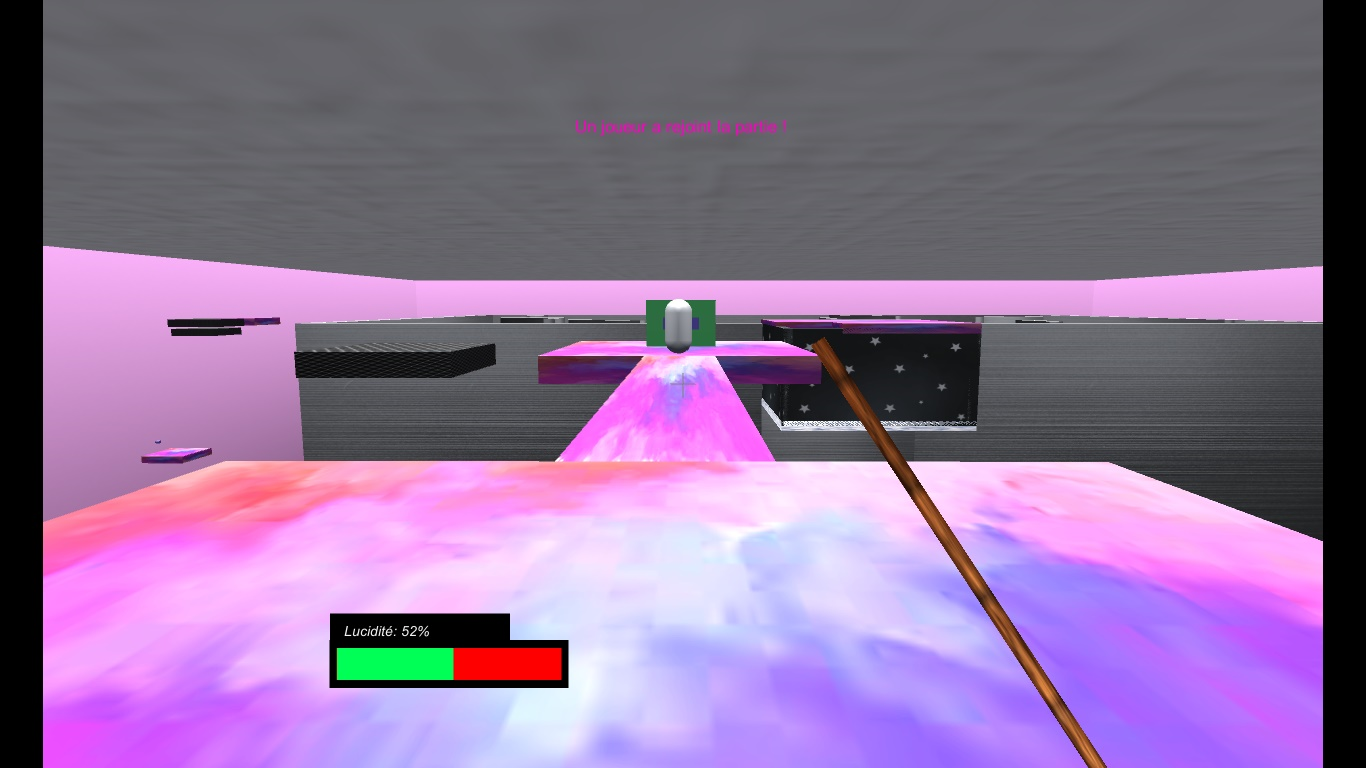
\includegraphics[scale = 0.4]{Multi.png}

\quad

\textit{Figure 6 : Mode multijoueur (2 joueurs connectés) }

\end{centering}

\quad

\quad

\newpage

	\subsection{Charles "gigi" GINANE :}


\quad

		\subsubsection{Ce qui a été fait :}


\quad

Pour cette deuxième soutenance, je me suis occupé du gameplay et aussi du son. 

Je me suis beaucoup attardé sur le son afin de pouvoir mettre une musique aux différents niveaux et de pouvoir avoir un jeu avec des bruitages et des sons (comme quand le joueur marche avec un bruit de pas par exemple). Pour cela j’ai dû créer un audioclip qui permet de jouer la musique en boucle et qui s’arrête dès que l’on ouvre le menu et qui reprend à sa fermeture à l’aide d’un script. J’ai ensuite developpé un gestionnaire de son avec différents bruitages son fonctionnement est simple, je donne un nom à chaque son dans une liste et chaque nom correspond à une musique et dès que le script trouve la musique, alors le son se lance. 


Je me suis pas mal servi du logiciel “Audacity” pour pouvoir adapter les sons au jeu afin d’éviter que les musiques soient trop lourdes pour le jeu ou alors adapter le son pour qu’on puisse l’entendre afin qu’il ne soit pas masqué par la musique du jeu.

J’ai dû faire face à quelques problèmes notamment certains sons qui empêchaient les autres d’être joués et qui posaient quelques problèmes. 
J’ai dans un second temps amélioré le gameplay, notamment le HUD comme je l’avais prévu, ce qui m’as permis aussi de m’occuper de la finalisation du projet.

Pour améliorer le HUD, j’ai tout simplement mis plus des textes à l’aide du UI (user interface) que j’ai mis sur le canvas spécial HUD. Ces textes permettent au joueur d’avoir des explications sur ce qu’il faut faire pour arriver au terme du niveau.


De plus, j’ai ajouté un texte qui met à jour les objectifs que le joueur doit accomplir pour pouvoir finir le niveau. Cela a pour but de guider le joueur tout au long du niveau.

J’ai mis un son qui permet de dire au joueur qu’il a accompli son objectif.

Ensuite, j’ai vérifié que les scripts marchaient bien pour tous les niveaux, que ce soit pour les sons ou pour le HUD.

J’ai donné pas mal d’idée à Marion pour la conception des niveaux du jeu. Ces idées ont été retenues pour la prochaine soutenance.

\quad
		\subsubsection{Ce qu'il reste à faire :}


Je ne suis pas en retard pour la deuxième soutenance, ce qui me reste à faire pour la dernière soutenance c’est de continuer à mettre de nouveaux sons notamment dans les différents niveaux, mettre différentes musiques.

J’améliorerai une fois de plus le gameplay pour qu’il soit le plus ressemblant possible à un jeu de réflexion notamment en affichant des textes sur les murs afin de mieux guider le joueur dans son parcours.


Enfin implémenter les derniers scripts relatifs aux textes qui s’affichent en haut de l’écran pour le solo et le multi qui permettent aux joueurs d’évoluer au sein des différents niveaux qu’ils contempleront.

		\subsubsection{Conslusion personnelle :}

Je suis assez satisfait du travail que j'ai fourni entre la première soutenance et la deuxième. J'ai pas mal avancé la partie son du projet ce qui permet un meilleur gameplay, cela m'as permis d’avoir plus de connaissance dans le domaine du gameplay et notamment des UI.

De plus, en implémentant le son, j'ai pu en apprendre beaucoup sur la façon d'implémenter un son et une musique et ses propriétes. J'en ai appris beaucoup sur la façon de gérer un son et éviter les problèmes qu'ils peuvent engendrer

\quad

\quad

\begin{centering}

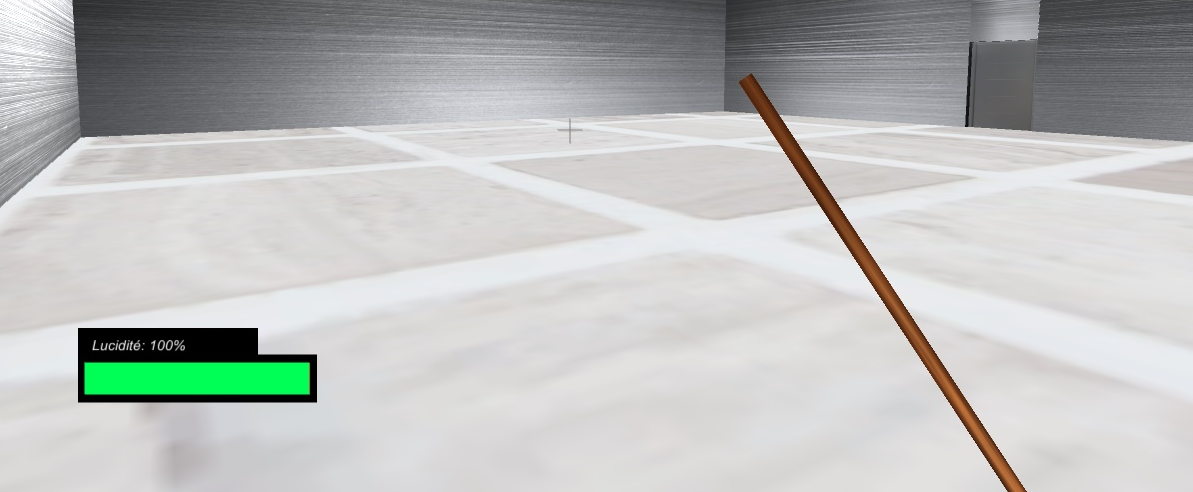
\includegraphics[scale = 0.4]{HUD.png}

\quad

\textit{Figure 7 : HUD }

\end{centering}

\quad

\newpage

	\subsection{Laurent "Aluxima" MARCHAUD :}

\quad



		\subsubsection{Ce qui a été fait :}

\quad 

\quad

En cette seconde phase d’avancement du projet, j’ai réalisé plusieurs choses. D’une part, la plus grosse partie du travail a été de créer un mode multijoueur en ligne pour notre jeu. Il a d’abord fallu créer les bases du multijoueur soit la connexion à un serveur et la gestion des connexions, la création d’une partie, la connexion entre les joueurs, les menus adéquats, etc. Une fois les bases du mode multijoueur mises en place, le plus difficile a été l’implantation de tous les éléments présents dans le mode solo dans le mode multijoueur. Cela pourrait paraître simple mais est en réalité bien plus compliqué que ce que je pensais. En effet, quasiment tous les scripts qui fonctionnaient dans le premier mode ne fonctionnaient plus en multijoueur, notamment à cause des relations entre les objets de la scène puisque l’on ne travaille désormais plus avec un seul joueur, mais avec tous ceux connectés.

De nouveaux éléments ont été rajoutés au mode solo et multijoueur, comme l’apparition de plateformes lorsque le joueur rentre en contact avec un certain point, lui permettant de poursuivre son niveau.

Je pense, comme ce que les étudiants des promotions précédentes nous ont conseillé, qu’il aurait plutôt fallu commencer notre jeu avec un mode multijoueur, puis de l’adapter pour le mode solo, car c’est dans ce sens qu’il y a le moins de changements à faire. Malheureusement, nous n’avions aucune connaissance en Unity avant le projet donc il aurait été difficile de commencer tout de suite par du multijoueur. Maintenant que je le sais, et que j’ai déjà acquis de bonnes bases en Unity, si je dois développer de nouveau un jeu, je commencerai par le mode multijoueur.

Avec la création d’un second niveau en mode solo, il a fallu créer un nouveau menu de sélection de niveaux et l’enregistrement de l’avancée du joueur. Une fois qu’il a terminé un niveau, il rejoint automatiquement, s’il existe, le prochain niveau et le succès est enregistré. Quand il reviendra dans le menu de sélection de niveaux, le bouton d’accès au menu suivant sera débloqué.

Comme prévu, et bien qu’il ait été déjà presque terminé avant la première soutenance, j’ai apporté quelques améliorations au site, comme la possibilité aux utilisateurs de laisser des commentaires, visibles par les autres.
Par ailleurs, l’acquisition du nom de domaine “lucidity.fr” s’est faite peu après la première soutenance, suivie de la migration du site complet sur mon serveur VPS, pour plus de sécurité, de fiabilité et de performance, puisqu’il était avant hébergé sur un Raspberry Pi sur mon réseau domestique.


\quad

\quad

\newpage
		\subsubsection{Ce qu'il reste à faire :}

\quad

\quad


Il reste énormément de choses à faire avant la dernière soutenance, comme l’amélioration du mode multijoueur avec notamment la création d’un système de “tchat” entre les joueurs et dans lequel le joueur verrait des informations du jeu comme la connexion d’un nouveau joueur, le succès d’une action, etc.

\quad

\quad

		\subsubsection{Conslusion personnelle :}

    Je suis satisfait du travail fourni par le groupe durant cette phase, et j’espère que cela continuera de la sorte jusqu’à la finition de notre jeu.

Personnellement, j’ai pu me familiariser avec le réseau de Unity, et je sens que le développement de ce jeu participe à l’amélioration de mes compétences en C\#, et en code en général !

\quad

\quad

\begin{centering}

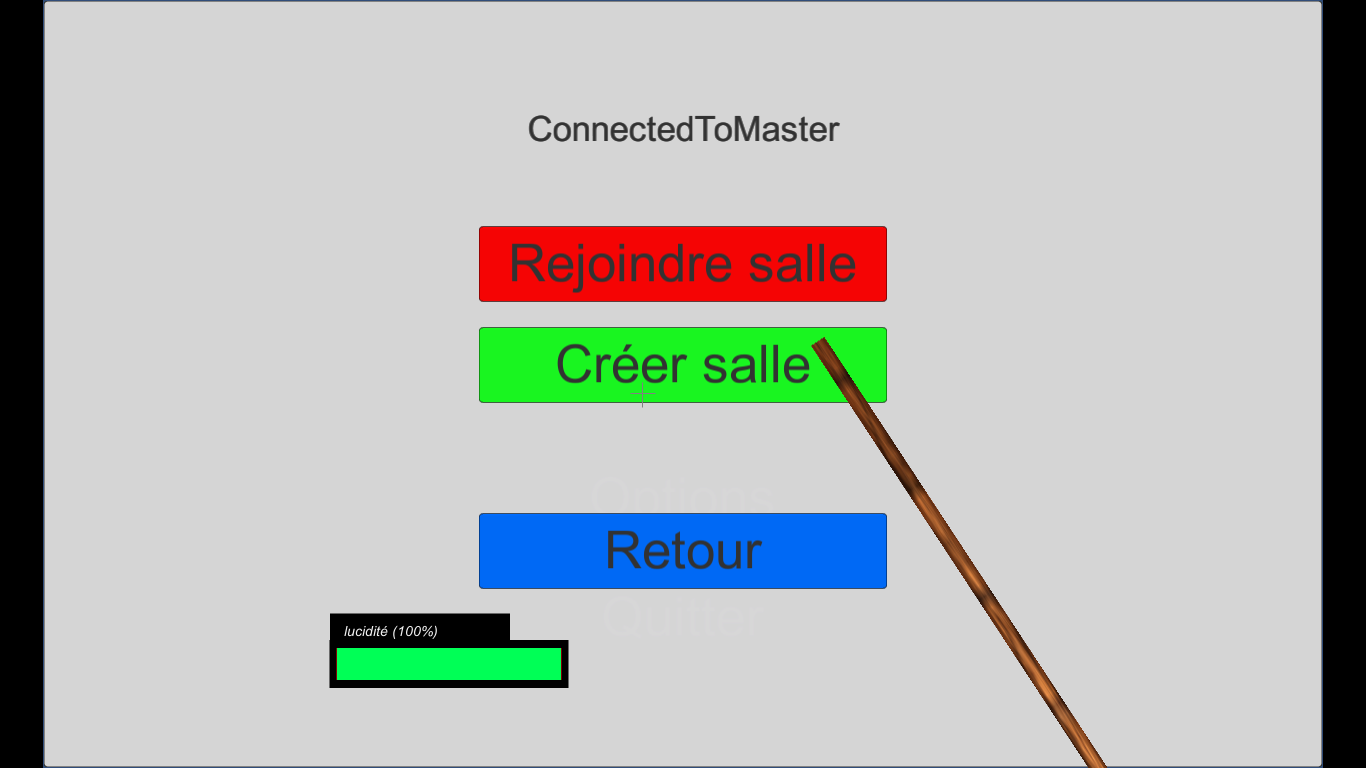
\includegraphics[scale = 0.4]{menumulti.png}

\quad

\textit{Figure 8 : Menu Multijoueur }

\end{centering}
\newpage

\section{Les objectifs pour la soutenance finale :}

\quad

\quad

Notre objectif principal va être de compléter  le plus possible notre jeu et d’ajouter un maximum de détails afin d’affiner notre projet. Pour le mode multijoueur, le but sera de rajouter un système de chat pour que les joueurs puissent communiquer par messages, ainsi que de faire des déplacements fluides pour les personnages. De plus, nous aurons un personnage comme joueur à la place de notre capsule. Au niveau des maps, il va falloir créer minimum deux maps pour avoir trois niveaux en mode solo et deux en multijoueur .Pour le gameplay, nous envisageons d’améliorer d’une part l’HUD en mettant plus de textes pour que le joueur soit le mieux guider possible, et d’autre part, mettre plus de son et plus de musiques aux niveaux déjà présents et aux futurs niveaux qui seront crées.


\quad

\quad

\underline{Légende de la figure 9 :} 

\quad
- = Non debuté

 \quad
+ = commencé 

\quad
++ = Avancement important 

\quad
+++ = Domaine fini

 \quad
\begin{centering}

			\begin{tabular}{|c|c|c|c|}
\hline Domaine &  3ème soutenance \\
\hline Moteur graphique & +++\\
\hline Moteur physique  & +++\\
\hline Site & +++\\
\hline Réseau & +++\\
\hline Gameplay &  +++\\
\hline Conception du monde & +++\\
\hline Son &  +++\\
\hline Finalisation &  +++ \\
\hline
			\end {tabular}

\quad

\textit{Figure 9 : Tableau d'avancement de la dernière soutenance}


\end{centering}

\quad

\quad

Evidemment, cela va de soi de dire que notre projet sera fini pour la dernière soutenance.
\newpage

\section {Notre ressenti par rapport à l'avancement du projet :}

\quad

\quad

Après avoir avoir fait le bilan avec l’ensemble du groupe, nous en avons conclu que les objectifs fixés par le cahier des charges pour la deuxième soutenance ont été respectés dans les délais imposés. Nous sommes donc confiants pour le reste du projet étant donné que nous n’avons aucun retard et que tout le dur travail que nous avons effectué est récompensé par un projet qui fonctionne.
Depuis le début nous avons un bon rythme et une bonne lancée qui nous permet d’avancer dans les temps sans se précipiter et de priviligier la qualité plutôt que de la quantité.

Grâce aux connaissances de chacun , l’entraide et la cohésion qui se sont formées entre les membres du groupe depuis le début du projet, nous avons pu avoir un bon ressenti pour la suite, c’est-à-dire, pour la soutenance finale.

\newpage

\section{Le multijoueur :}

\quad

    La création d’un mode multijoueur dans notre jeu a été la partie la plus difficile dans notre projet. Il a d’abord fallu choisir une extension de Unity pour gérer tout cela. Nous avons choisi le plugin “Photon Unity Network” qui utilise le système multijoueur de base de Unity, mais qui le simplifie énormément. Ce système nous offre la possibilité d’héberger sur leurs serveurs nos parties en ligne avec un maximum de 20 connexions simultanées et 500 messages par seconde, les messages étant toutes les informations échangées entre les joueurs connectés, comme les informations de position, de connexion, et tout ce qui peut être échangé entre les joueurs. 

    La première étape a été la création d’un menu avec 2 boutons: un pour rejoindre aléatoirement une partie en ligne existante, et l’autre pour créer une salle que d’autres joueurs pourront rejoindre. Nous avons créé un compte gratuit sur le site du plugin Photon Network, qui nous a fourni un identifiant unique nous permettant de créer nos propres salles. Tout ce qui est connexion, création de salles, déconnexions, transfert d’hôte est automatique avec Photon. En effet, lorsqu’un joueur crée une salle, il est l’e “maître” de celle-ci. Quand un autre joueur se connecte, le premier reste le maître de la salle, mais si le maître se déconnecte, c’est un autre joueur qui présent dans la salle qui  passe maître. Quand il n’y a plus personne dans la salle, c’est-à-dire lorsque le dernier joueur s’y déconnecte, la salle se détruit automatiquement et on ne peut plus la rejoindre. Tout cela est donc géré quasiment automatiquement par Photon.

    Ensuite, nous avons dû faire en sorte que les joueurs présents dans la même salle soient parfaitement synchronisés. Ce n’est pas la seule synchronisation à faire, il y avait aussi celle des plateformes qui bougent en même temps sur les clients, et les objets qui s’instancient à partir des joueurs et qui sont envoyés aux autres joueurs connectés. Toutes les synchronisations sont faites avec des mouvements fluides sauf celles du personnage que l’on a pas encore réussi à implementer. Tous les scripts ont dû être adaptés au multijoueur, notamment à cause des problèmes d’instanciation. En mode solo, instantiation était immédiate car on travaillait avec un seul joueur facile à trouver. Désormais, les joueurs sont multiples et tous les scripts en dépendant doivent trouver le bon joueur. Par exemple, pour le système de pause du jeu, on arrêtait simplement le temps et tous les objets s’arrêtaient de bouger jusqu’à ce qu’on quitte la pause et que le temps revienne à la normale. Sauf qu’en multijoueur, on ne veut pas que les objets s’arrêtent de bouger quand un joueur est en pause, on a donc dû changer ce système, comme bien d’autres.

    Des textes d’indication de connexion et déconnexion des joueurs sont présents. Un texte s’affiche quand un joueur se connecte ou déconnecte. Nous pensons inclure ces messages dans le système de “chat” pour plus de clarté.



\newpage

\section{conclusion}

\quad

\quad

C’est donc dans une bonne ambiance de travail que notre projet continue. Ainsi notre jeu est maintenant jouable en mode solo et en multijoueur. Cependant il nous reste encore des modifications à apporter pour avoir un jeu complet. 

Ce projet est très instructif, que ce soit au niveau code ou bien relationnel. En effet le travail de groupe n’est pas toujours aussi facile que ce qu’on pourrait penser, bien que notre groupe s’en sort plutôt bien.

Bien que le projet avance bien, il n’est pas encore fini. Il nous faut donc continuer dans notre lancée et le terminer.

\quad

\quad

\end{document}